\documentclass[letterpaper, 10pt]{article}
\usepackage[psamsfonts]{amssymb}
\usepackage{amsmath, amsthm, anysize, enumerate, color, graphicx}
\usepackage{amssymb,amsbsy, amsthm, amsmath, amstext, amsopn}
\usepackage[colorlinks,
            %linkcolor=black!50!red,
            citecolor=blue,
            pdfpagemode=None]{hyperref}
\usepackage{cleveref}

\newtheorem{theorem}{Theorem}[section]
\newtheorem{question}[theorem]{Question}
\newtheorem{problem}[theorem]{Problem}
\newtheorem{corollary}[theorem]{Corollary}
\newtheorem{conjecture}[theorem]{Conjecture}
\newtheorem{lemma}[theorem]{Lemma}
\newtheorem{proposition}[theorem]{Proposition}
\newenvironment{proof_of}[1]{\noindent {\bf Proof of #1:}
	\hspace*{1mm}}{\hspace*{\fill} $\qedsymbol$ }
\newcommand{\widgraph}[2]{\includegraphics[keepaspectratio,width=#1]{#2}}

% % the following creates defns with the usual roman font, not in italics
\newtheorem{definition}{Definition}[section]
\newtheorem{fact}{Fact}[section]

% Not in italics
\theoremstyle{definition}
\newtheorem{remark}[theorem]{Remark}
\newtheorem{example}[theorem]{Example}

% Notational convenience
\newcommand{\E}{\mathbb{E}}
\newcommand{\R}{\mathbb{R}}
\newcommand{\N}{\mathbb{N}}
\newcommand{\Q}{\mathbb{Q}}
\renewcommand{\P}{\mathbb{P}}
\newcommand{\M}{\mathcal{M}}
\newcommand{\W}{\mathcal{W}}
\newcommand{\sgn}{\text{sgn}}
\newcommand{\conv}{\text{conv}}
\newcommand{\Dom}{\text{Dom}}
\newcommand{\stirlingtwo}[2]{\genfrac{\lbrace}{\rbrace}{0pt}{}{#1}{#2}}

\begin{document}

\title{Bispectral group invariants for data science}
\author{Et al., Christopher Hillar\thanks{Redwood Center for Theoretical
    Neuroscience, \texttt{chillar@msri.org}.}, Et al. \hspace{20mm}}

\maketitle

\begin{abstract}
We motivate using bispectral invariants for understanding data up to natural transformations of the underlying coordinate space.  Often, orbits under such natural ``relabellings" of data are large sets yet nonetheless need to be identified as single clusters in applications.  One solution is to determine a complete set of invariants; that is, a map to a metric space having the following two properties: (1) all points in an orbit map to the same invariants, and (2) distinct orbits are mapped differently.  We advocate determining complete sets of invariants by utilizing the machinery of an object called the bispectrum, which can be effectively computed using the concrete representation theory of the underlying transformation group.  We present several examples of the theory and discuss potential applications to real-world problems.
\end{abstract}

%---------
\section{Introduction}
\label{Sec:Intro}

We investigate objects called \textit{bispectrums}, a general construction of features that do not change when data are acted upon by a transformation group.  Although invariant theory is a classical topic in pure mathematics, a direct application of the bispectrum concept first appears in work by statistician John Tukey to define higher-moments of time-series that can detect non-Gaussian phenomena \cite{tukey1953spectral}.  We became aware of them from Kondor's applications to machine learning \cite{kondor2007complete, kondor2008thesis, kondor2008skew}, which, in turn, were inspired by papers of Kakarala \cite{KakaralaPhD, KakaralaTriple}.  We note that many independent groups continually rediscover this circle of ideas \cite{gourd1989methode}, even today \cite{cohen2018spherical}.

More remarkably to us, however, already in 1947, considerations from neuroscience theory -- predating experimental evidence of ``complex cells" from recordings in visual cortex -- lead researchers to the idea of bispectra for canonical representations (``universality") in sensory coding \cite{pitts1947}; see Figure \ref{pitts_bispectra}.

\subsection{Group invariants}

Let $G$ be a \textit{group}, which abstractly means that it is a set with a binary (``multiplication") operation $\cdot: G \times G \to G$, usually denoted $(g_1,g_2) \mapsto  g_1 \cdot g_2$, satisfying the axioms: (1) associativity, (2) there is an identity element, and (3) inverses exist. Groups are ubiquitous.  For instance, the integers $\mathbb Z$ under addition $+$ form a group; in fact, an \textit{commutative} group, which has the additional property that multiplication is symmetric ($g_1\cdot g_2 = g_2\cdot g_1$).  The set of ``integers modulo $n$" is also a classical example of a group: $\mathbb Z / n\mathbb Z = \{0, 1, \ldots, n-1\}$.  

Another commutative group is the (continuous) set of nonzero complex numbers $\mathbb C^* := \mathbb C \setminus \{0\}$ under scalar multiplication.  More interesting are the non-commutative \textit{general linear} groups $GL_n(\mathbb C)$, which consist of all invertible $n \times n$ matrices with entries in the complex numbers $\mathbb C$:
\[ GL_n(\mathbb C) := \{ M \in \mathbb C^{n \times n}: \det(M) \neq 0\}.\] 

Chronologically, the theory of groups was only formalized systematically after being concretely worked on in the form of collections of ``transformations" on some underlying geometric set.  For instance, the group of (distance-preserving) orthogonal $2 \times 2$ real matrices taking a square in the plane to itself is such an example object studied by these early theorists.  In this case, one can check that there are $8$ such matrices, or \textit{symmetries}, and they are in correspondence with elements of the (non-commutative) \textit{dihedral group} $D_4$:
\[ \left\{\left[\begin{array}{cc}1 & 0 \\0 & 1\end{array}\right], \left[\begin{array}{cc}0 & -1 \\ 1 & 0\end{array}\right],
\left[\begin{array}{cc}-1 & 0 \\0 & -1\end{array}\right],\left[\begin{array}{cc}0 & 1 \\-1 & 0\end{array}\right],
\left[\begin{array}{cc}-1 & 0 \\0 & 1\end{array}\right],\left[\begin{array}{cc}0 & 1 \\1 & 0\end{array}\right],
\left[\begin{array}{cc}1 & 0 \\0 & -1\end{array}\right],\left[\begin{array}{cc}0 & -1 \\-1 & 0\end{array}\right] \right\}.\]

More generally, one can consider the collection of all finite groups.  Somewhat surprisingly, only recently has a complete classification of all such objects been carried out \cite{gorenstein2013finite}.  The main difficulty (an effort involving thousands of research pages) was ruling out the existence of more ``sporatic" groups not on a known list (the largest, called the ``monster group", having size $\sim 8 \cdot 10^{53}$).  Although finite groups can be very complex, there is nonetheless a master class of groups containing them all.  These are the \textit{symmetric} groups $S_n$, also called \textit{permutation} groups.  Concretely, they are the set of \textit{bijections} $\pi$ from an $n$-element set $[n] := \{1, 2, \ldots, n\}$ to itself; i.e., those maps $\pi: [n] \to [n]$ that are both injective and surjective.  Multiplication $\cdot$ in this group is simply composition of maps $\tau \cdot \pi = \tau \circ \pi$.  The following fact explains why $S_n$ is a fundamental set of groups.

\begin{theorem}[Cayley's Theorem]
Every finite group is the subgroup of some permutation group.  I.e., given any finite group $G$, there is a big enough integer $n$ such that $G$ is a subgroup of $S_n$.  
\end{theorem}
Another way of explaining Cayley's theorem is that all finite groups just eventually pop out of nowhere as subgroups of $S_n$ as $n$ increases.
It turns out that $n = |G|$ (the size of $G$) is sufficient in this theorem. 

\begin{figure}[t!]
 \begin{center}
a)  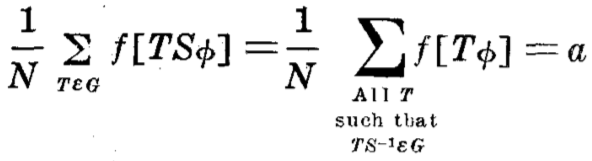
\includegraphics[width=.45 \linewidth]{figs/pitts_1947_first_bispect_coeff.png}  
b) 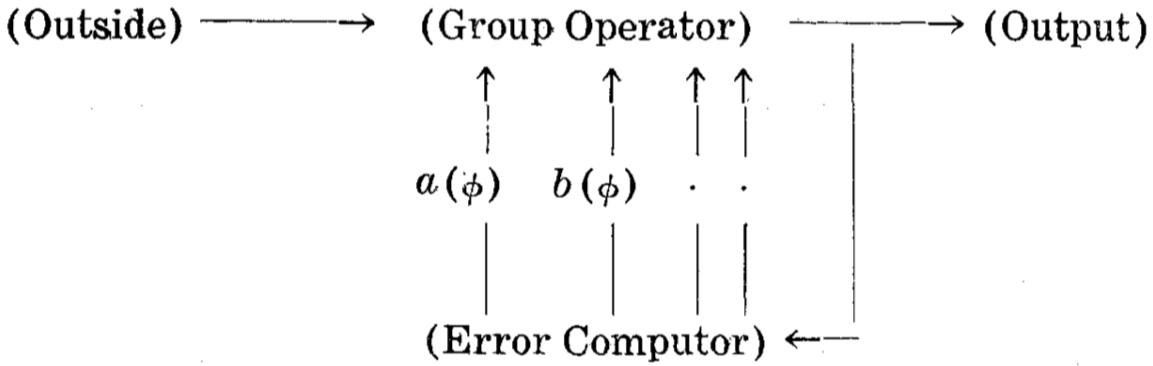
\includegraphics[width=.45 \linewidth]{figs/pitts_1947_diagram.png}   
\caption{\textbf{Universality in sensory neuroscience first motivation for bispectra}. a) The simplest bispectral coordinate representing part of a universal sensory signal representation, and b) Neural circuity schematic for computation of universal representations of sensory measurements (see \cite{pitts1947} for more details).}
\label{pitts_bispectra}
\end{center}
\end{figure}

\begin{figure}
 \begin{center}
  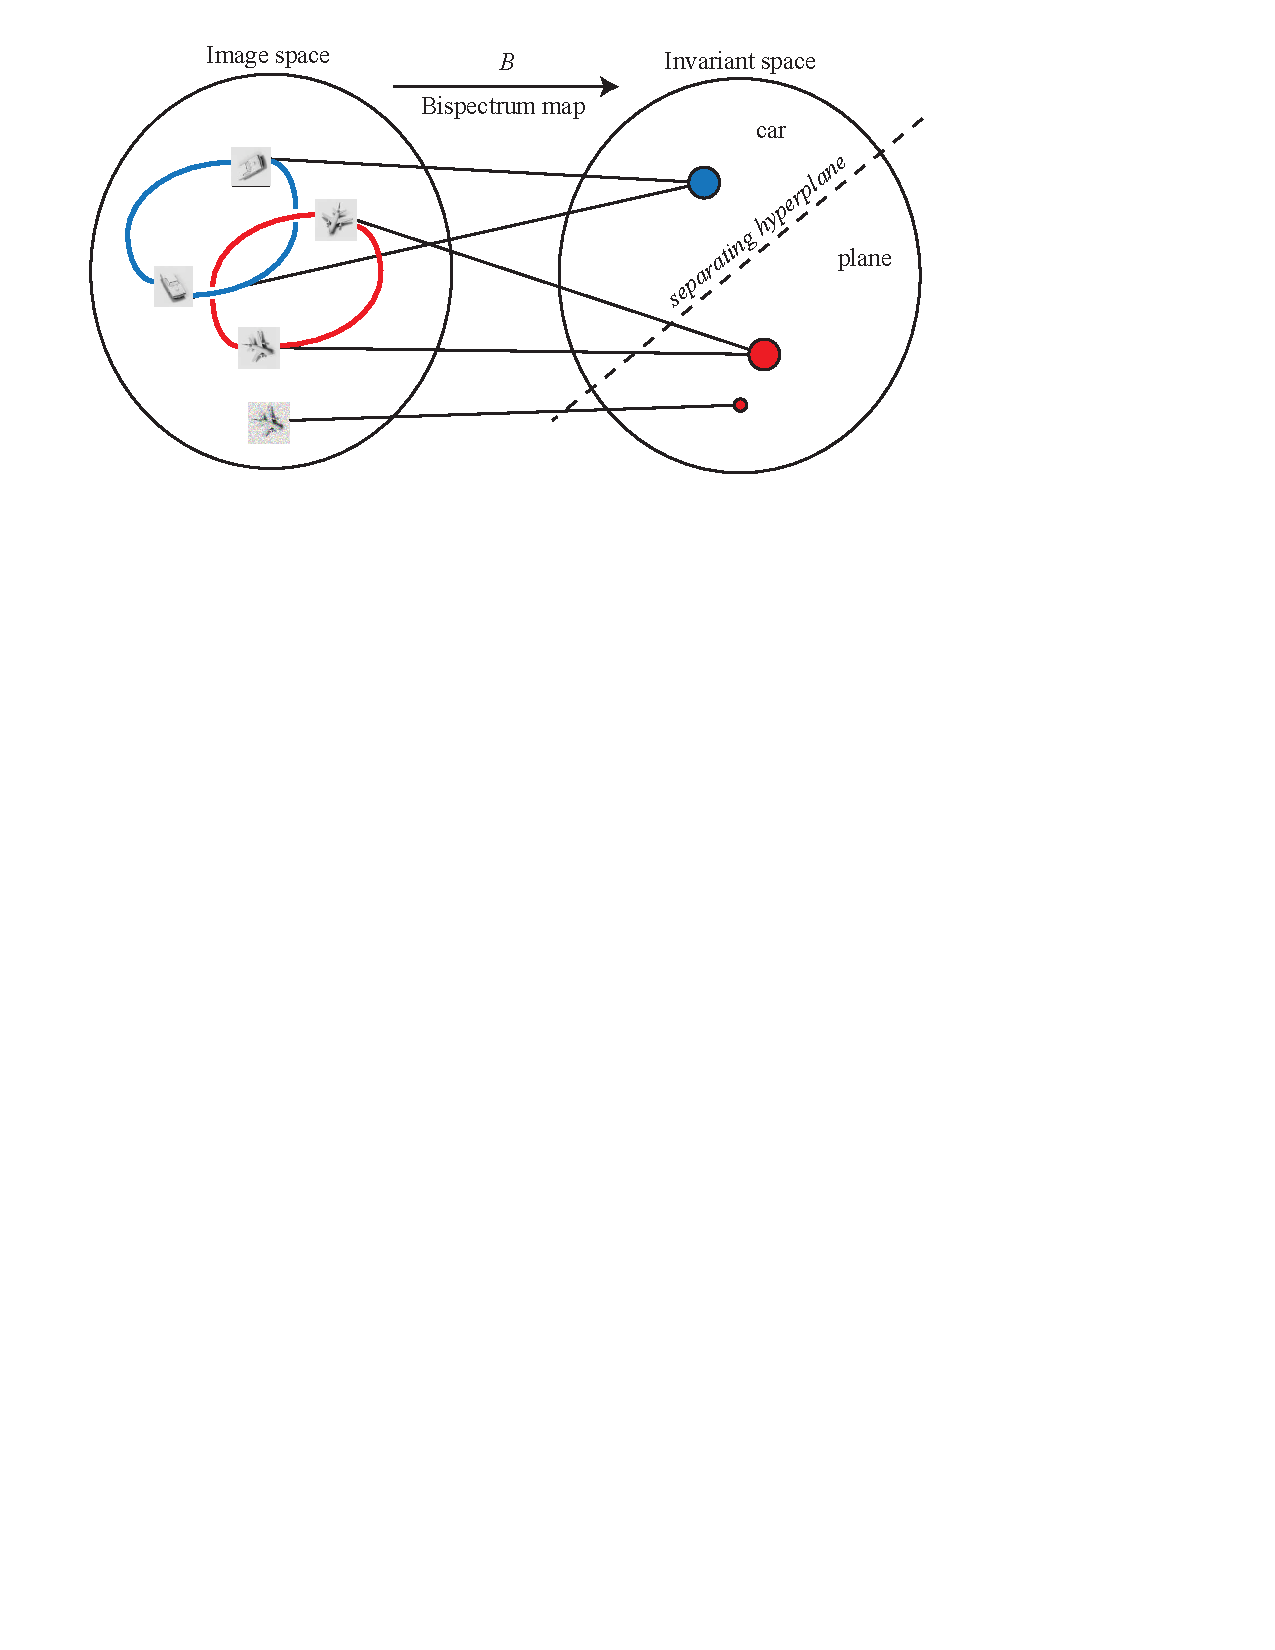
\includegraphics[width=.8 \linewidth]{figs/bispectrum2.pdf} 
\caption{\textbf{Clustering orbits in the space of bispectra}. Cartoon depicting intuition of how one could use a rotationally invariant bispectrum map for object discrimination in the space of images.  After computing a one-time continuous preprocessing mapping, translations and rotations of an object map to single points, making it easier to discriminate between them using standard hyperplane classifiers.}
\label{bispetrum_intuition}
\end{center}
\end{figure}

Recall from above that a classical concern were those transformations $T$ in a group $G$ (e.g., the $2 \times 2$ orthogonal group $O(2)$) that fix a particular subset of some data space $X$ (e.g., the square as one particular subset of the plane). %; that is, special focus was given to the set $\{T \in G: T\mathbf{x} = \mathbf{x}\}$.
However, from the perspective of neuroscience and machine learning, it is often the case that a more important object in practice is the \textit{orbit} $G\mathbf{x}$ of a given datapoint $\mathbf{x}$; that is, the following subset of the ambient space $X$ generated by moving $\mathbf{x}$ around by acting on it with arbitrary elements of the group:  
\[ G\mathbf{x} := \{g\cdot \mathbf{x}: g \in G\} \subseteq X.\]
In Figure \ref{bispetrum_intuition}, an example of this concept is the (red) collection of all rotations of a specific toy plane in 2D.

This brings us to our main concern here: how to construct readily computable invariant features in a space? 
The notion of ``group invariant" is quite old, but maybe most notably motivated by physics: invariants often come in the guise of ``conservation laws" (for instance, derived from Noether's theorem  \cite{noether1918invariante}).  Intuitively, these laws take the form $\forall g \,E(g \cdot \mathbf{x}) = C$ for some function $E$ of the underlying coordinates and some constant $C$ independent of transformation $g \in G$.  For instance, the energy of a box should not change if it has only been rotated in space.


\subsection{Construction of bispectra}

A clear and succinct exposition of what takes place in this construction can be found in \cite{kondor2007complete}.
The main thing to note is that a main part of the computation is to decompose a tensor of two representations into its constituent parts, the same mathematics of which is used to determine particles emerging from supercollider smashings. 

\begin{figure}
\begin{center}
a)  
\includegraphics[width=.3 \linewidth]{figs/hobbes_amplitude_hobbes_phase.png} 
b) 
\includegraphics[width=.3 \linewidth]{figs/calvin_amplitude_calvin_phase.png} 
 c) 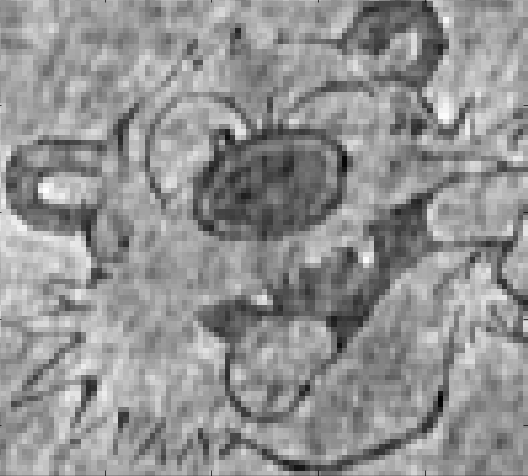
\includegraphics[width=.3 \linewidth]{figs/calvin_amplitude_hobbes_phase.png}  
\caption{\textbf{Fourier power is an insufficient invariant}. a) Hobbes, b) Calvin, c) Calvin's 2D Fourier Amplitudes with Hobbes Phases.}
\label{swap_phase_calvin}
\end{center}
\end{figure}

It is important to note here that classical invariants such as Fourier power do not capture all of the invariant information in the signal.  For instance, consider Figure \ref{swap_phase_calvin}, in which we have two very distinct images yet with the same Fourier amplitudes.
This is a major reason to explore higher-order features of data.

Intuition for bispectra can be found in the illustration given in Figure \ref{bispetrum_intuition}.  One would like a method for collapsing many versions of a canonical object into one.  

\subsection{Bispectra for data science}

The basic idea here is that more complete sets of invariants should be useful.  For instance, consider the toy example of trying to recover a Calvin image from many translated, noisy measurements of him.  Averaging in original pixel space won't work and Fourier power is not strong enough to capture the original.  The solution is to ``average in bispectrum space and invert"; see Figure \ref{bispetrum_invert_calvin}.
Compare with figures 3 and 4 from \cite{sadler89}.

Another powerful perspective with which to view bispectral invariants is that they remove quantifiers in object classification tasks.  More specifically, consider the problem of finding the ``distance" between two points ``up to the group".  Naively, this involves an optimization of the form (so-called ``template matching"):
\[ \min_{g, \,h \in G} || g \cdot \mathbf{x} - h\cdot \mathbf{y}||.\]
On the other hand, with a bispectrum $\beta$ on call, a metric space comparison without the quantifier over the group becomes the simple expression:
\[d(\mathbf{x}, \mathbf{y}) = || \beta(\mathbf{x}) - \beta(\mathbf{y})||.\]
In many instances (when $\beta$ forms a complete set of invariants), this distance is zero if and only if $\mathbf{y}$ is a group translation of $\mathbf{x}$; that is, when there exists a $g \in G$ with $\mathbf{x} = g \cdot \mathbf{y}$.  In any case, however, $d$ is a distance between orbits and can be used with any classical machine learning method (nearest neighbor, SVMs, etc.) to extract invariant structure.

Sometimes the savings by removing the ``$\min$" quantifier as above can be enormous.  Take, for instance, the problem of determining how close two weighted graphs are to each other up to ``relabelling" of the vertices (see Figure \ref{bispetrum_graphs}).  With the naive approach, a graph on $v$ vertices has up to $|S_v| = v!$ other graphs in its orbit.  Thus, the bispectrum approach has the potential to speed up computations by a factor of $v!$.

\subsection{Bispectra for neuroscience}

A very preliminary study of the correlation between neural responses in V1 took place in \cite{Mudigonda13}.



%---------
\section{General theory}
\label{Sec:General}


\section{Examples}

\subsection{1D Bispectra}

The bispectrum of a one dimensional signal is the Fourier transform of its triple correlation, and it is invariant under time translations.



\begin{figure}
\begin{center}
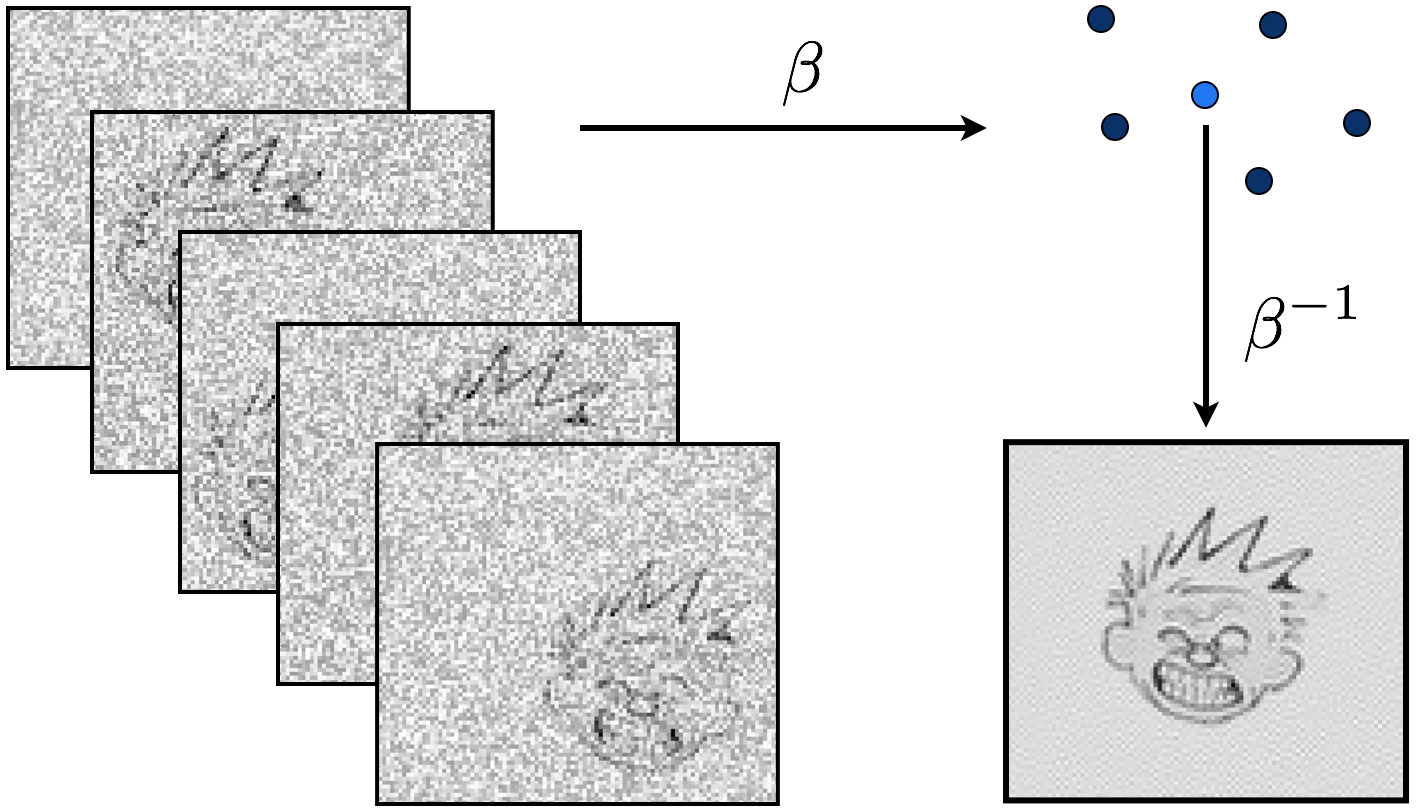
\includegraphics[width=.9 \linewidth]{figs/calvin_inv_bispectrum.png} 
\caption{\textbf{Inverting the 2D bispectrum}. By averaging noisy translated Calvins in the bispectrum space and inverting, we can uncover the original.}
\label{bispetrum_invert_calvin}
\end{center}
\end{figure}


%\begin{figure}
%\begin{center}
%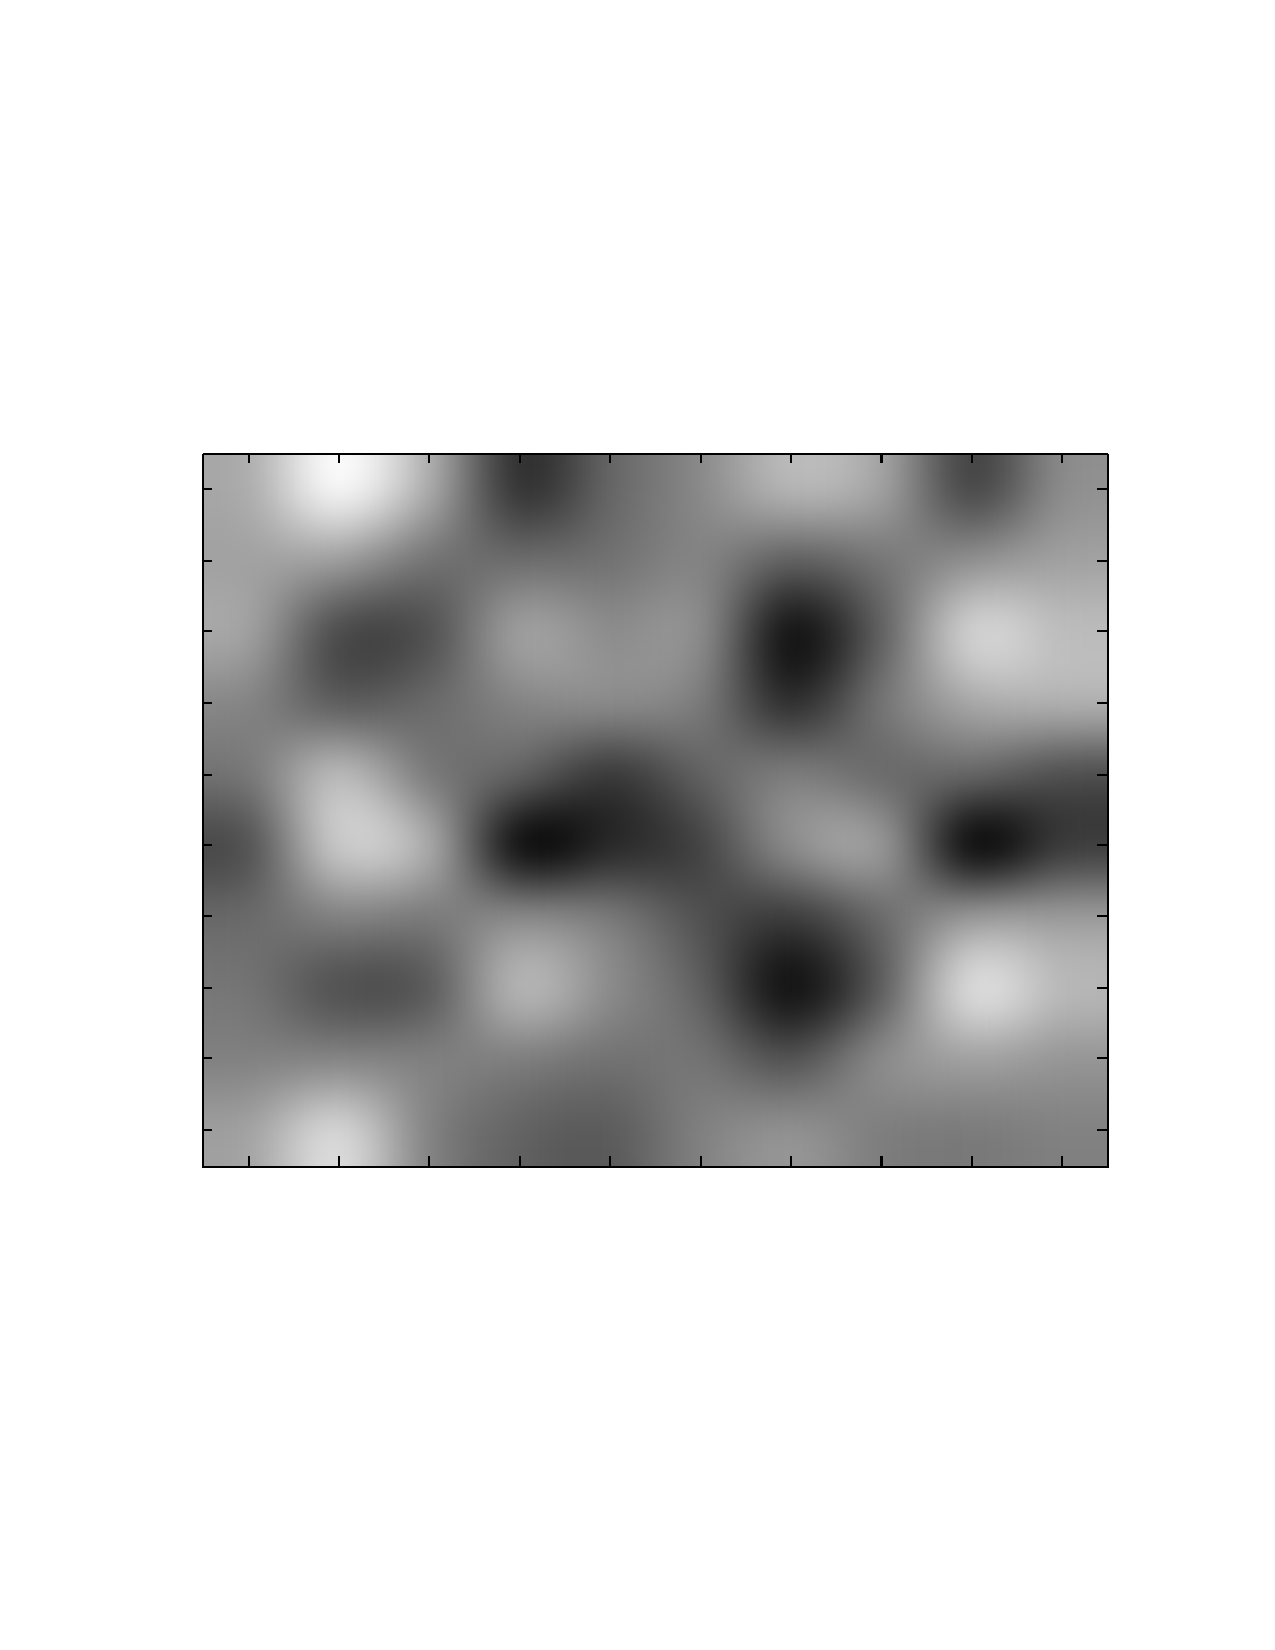
\includegraphics[width=.2 \linewidth]{figs/avg_bispec_real_cell25.pdf} 
%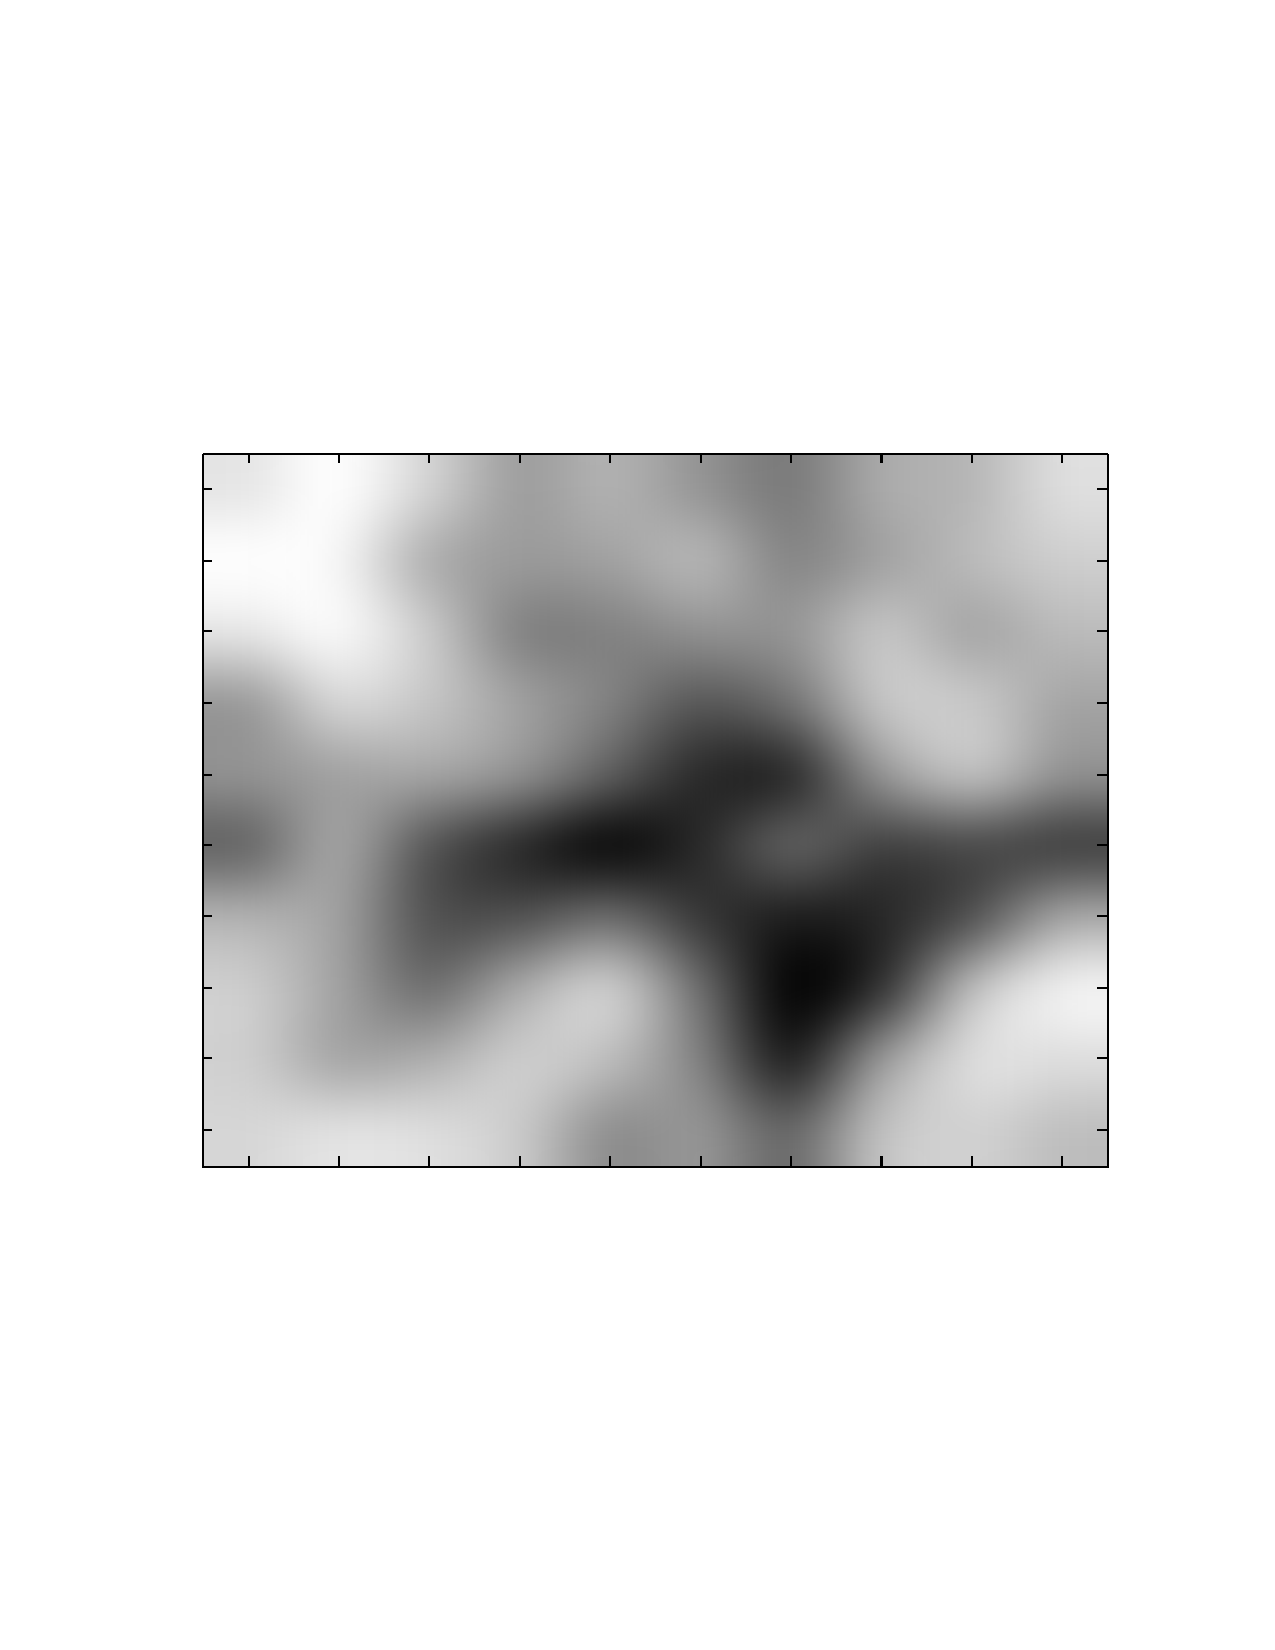
\includegraphics[width=.2 \linewidth]{figs/avg_bispec_real_cell30.pdf} 
%\caption{\textbf{Recovering invariant neuron responses}. For two cells, inverses of the spike-triggered bispectral averages.}
%\label{bispetrum_intuition2}
%\end{center}
%\end{figure}
% 


\begin{figure}
\begin{center}
   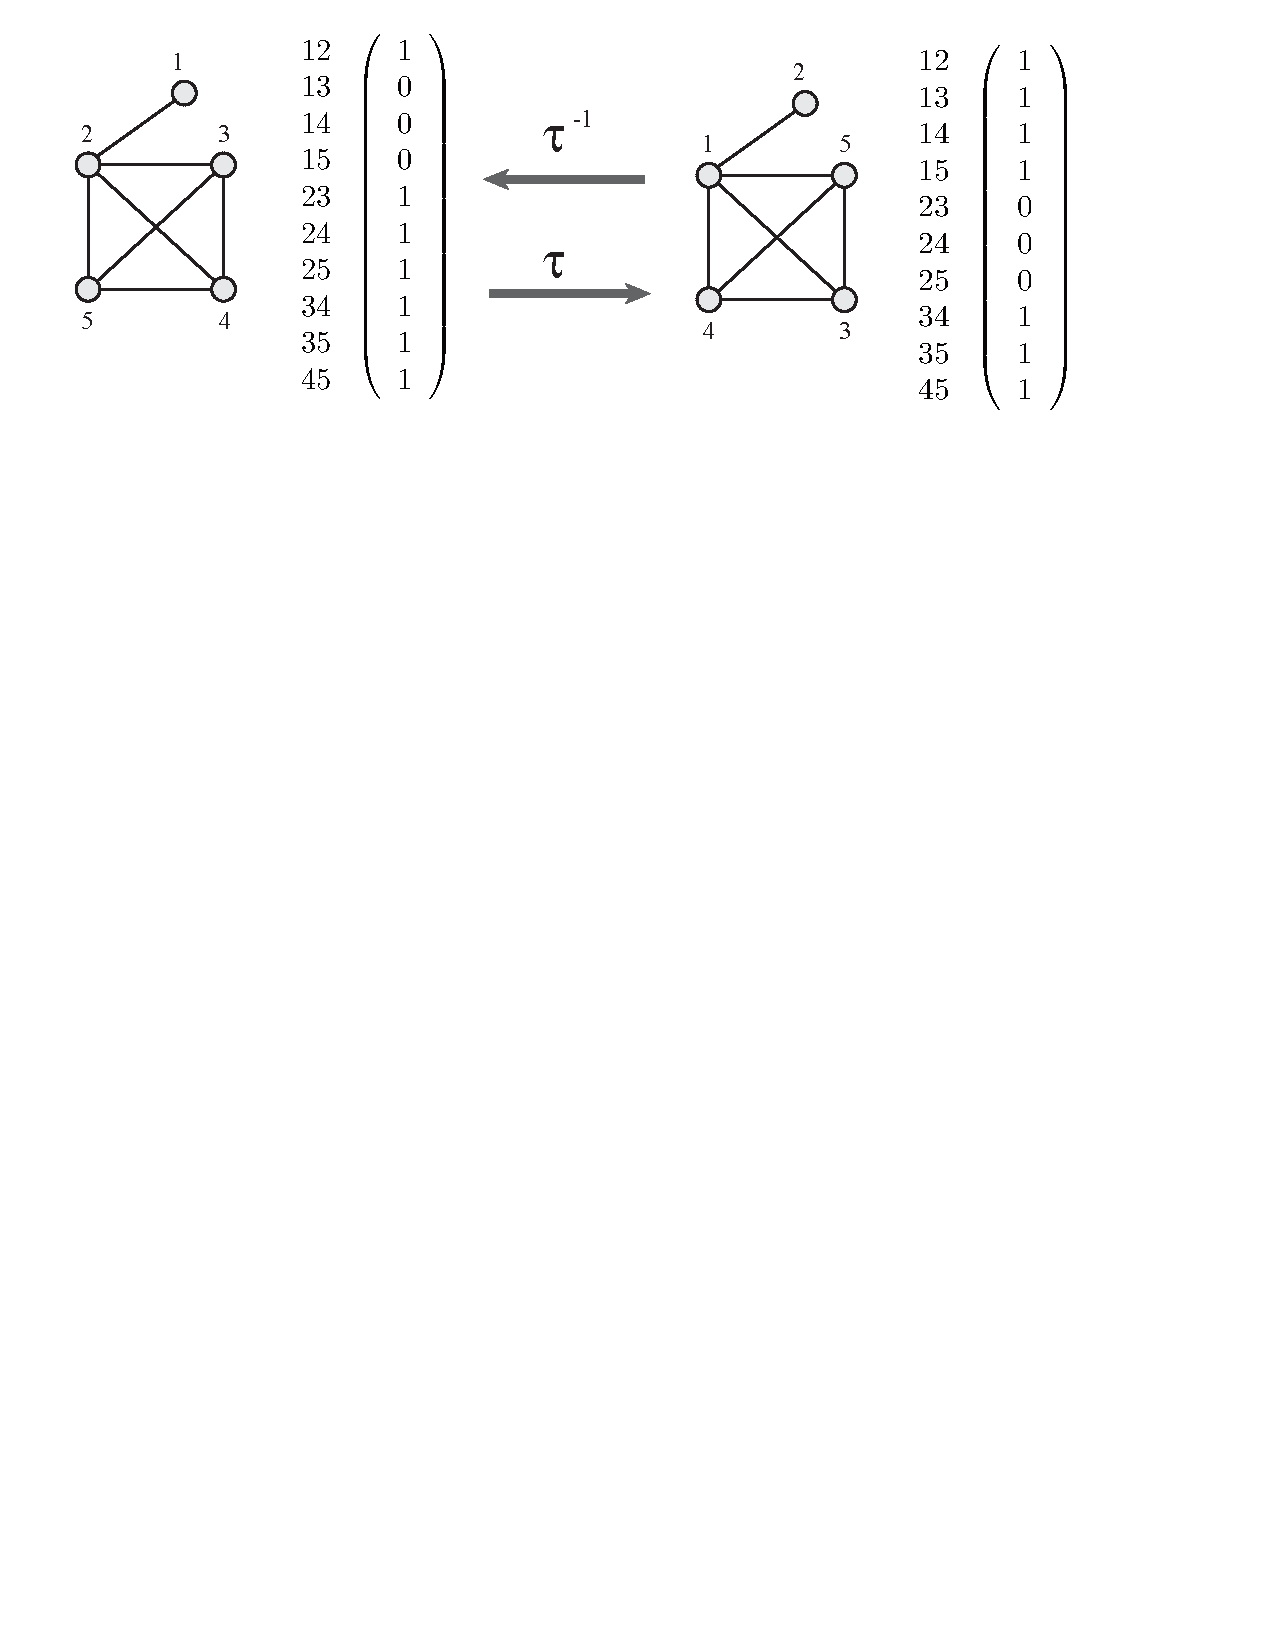
\includegraphics[width=.85 \linewidth]{figs/binary_graph.pdf} 
\caption{\textbf{The graph bispectrum}. The problem of graph isomorphism can be seen as one of finding a complete set of invariants, i.e. bispectra.}
\label{bispetrum_graphs}
\end{center}
\end{figure}


\begin{figure}
\begin{center}
   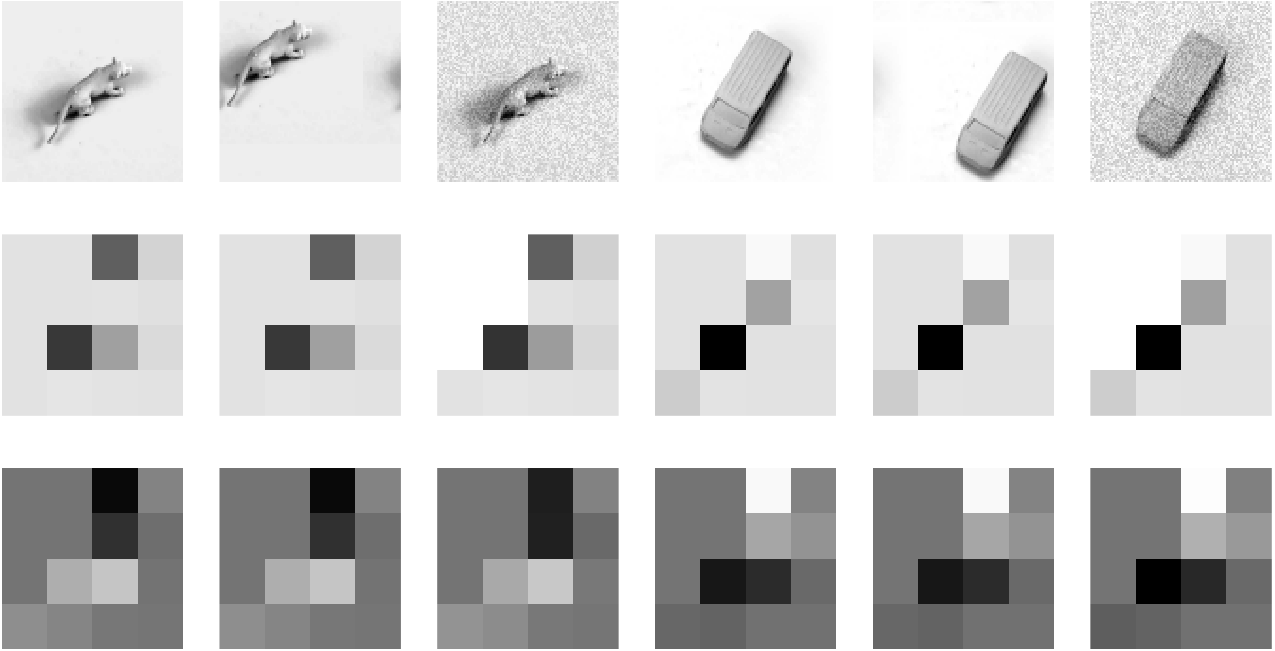
\includegraphics[width=.9 \linewidth]{figs/bispect_examples_2.png} 
\caption{\textbf{2D translationally invariant features}. In row \textbf{a}, we show 6 different images:  from left to right, we have a toy cat, a translated toy cat, a noisy cat, and the same for a toy truck.  For each image, we computed 16 complex-valued bispectrum features. The real parts \textbf{b} (imaginary parts \textbf{c}) of these features are depicted as a colormap with white representing the value 3000 and black, -2400.  Note the features are invariant to translations and retain salient structure even after corruption.}
\label{bispetrum_intuition2}
\end{center}
\end{figure}



\subsection{2D Bispectra}

\begin{figure}
 \begin{center}
   \includegraphics[width=\linewidth]{figs/linesbispectrum.png} 
\caption{\textbf{2D bispectrum}. For 3 different images (top left), displayed are Fourier power (top right) and 2D bispectrum (bottom).}
\label{bispetrum_2dex}
\end{center}
\end{figure}

\subsection{$n$D Bispectra}

\subsection{Spherical Bispectra}

To better discuss its invariance properties, we also explain previous results \cite{kondor2007complete} for a toy dataset consisting of randomly rotated and translated images from the MNIST dataset \cite{lecun1998mnist}.  The original images are size $28\times 28$, but most of them only occupy a fraction of the image patch. The characters are rotated by a random angle between 0 and $2\pi$, clipped, and embedded at a random position in a $30\times 30$ patch.  2-class SVMs were trained for all possible pairs of digits. As a baseline, SVMs with linear kernels were used on the original 900-dimensional pixel intensity vector.  This was compared to similar linear SVMs on the bispectrum features. 

\begin{table}[t]
  \tiny
  \centering
  \begin{tabular}{|l|l|l|l|l|l|l|l|l|l|l|}
\hline
&1&2&3&4&5&6&7&8&9\\
\hline
0&${\textbf{0.8}(0.4)}$&${\textbf{6.2}(2.4)}$&${\textbf{5.1}(1.5)}$&${\textbf{5.0}(1.1)}$&${\textbf{2.9}(1.5)}$&${\textbf{4.1}(2.4)}$&${\textbf{2.7}(1.1)}$&${\textbf{5.0}(1.6)}$&${\textbf{5.9}(2.9)}$\\
&${17.1(3.7)}$&${33.9(3.6)}$&${42.1(3.6)}$&${30.6(2.5)}$&${37.8(3.5)}$&${31.4(5.9)}$&${29.4(3.8)}$&${42.6(4.3)}$&${27.6(3.2)}$\\
\hline
1&&${\textbf{0.7}(0.8)}$&${\textbf{0.4}(1.0)}$&${\textbf{3.1}(1.3)}$&${\textbf{0.0}(0.0)}$&${\textbf{1.4}(0.9)}$&${\textbf{1.8}(1.5)}$&${\textbf{2.7}(2.0)}$&${\textbf{1.0}(1.0)}$\\
&&${30.8(2.9)}$&${29.3(4.5)}$&${35.0(3.4)}$&${30.7(2.9)}$&${34.5(4.5)}$&${38.3(4.1)}$&${24.6(2.6)}$&${34.8(3.6)}$\\
\hline
2&&&${\textbf{15.9}(5.8)}$&${\textbf{15.8}(3.2)}$&${\textbf{8.1}(3.6)}$&${\textbf{9.6}(2.0)}$&${\textbf{11.1}(2.3)}$&${\textbf{9.3}(1.6)}$&${\textbf{10.6}(3.0)}$\\
&&&${49.1(4.2)}$&${47.1(4.7)}$&${45.2(4.3)}$&${51.4(5.2)}$&${47.2(5.5)}$&${47.4(6.2)}$&${46.7(3.0)}$\\
\hline
3&&&&${\textbf{4.8}(1.7)}$&${\textbf{16.4}(5.7)}$&${\textbf{7.5}(2.8)}$&${\textbf{4.0}(1.1)}$&${\textbf{10.7}(3.8)}$&${\textbf{7.7}(3.0)}$\\
&&&&${44.6(3.0)}$&${49.1(4.8)}$&${49.4(5.3)}$&${44.7(4.4)}$&${50.4(4.2)}$&${47.6(5.6)}$\\
\hline
4&&&&&${\textbf{6.3}(1.9)}$&${\textbf{10.9}(4.1)}$&${\textbf{15.0}(2.9)}$&${\textbf{6.3}(3.6)}$&${\textbf{17.0}(1.8)}$\\
&&&&&${40.1(6.7)}$&${50.1(5.3)}$&${45.3(3.3)}$&${46.3(2.6)}$&${49.8(4.7)}$\\
\hline
5&&&&&&${\textbf{14.6}(2.4)}$&${\textbf{5.3}(2.3)}$&${\textbf{6.6}(2.7)}$&${\textbf{6.8}(2.2)}$\\
&&&&&&${50.0(4.0)}$&${41.7(4.1)}$&${44.6(3.3)}$&${46.0(4.4)}$\\
\hline
6&&&&&&&${\textbf{7.7}(4.1)}$&${\textbf{9.0}(2.9)}$&${\textbf{20.2}(3.6)}$\\
&&&&&&&${48.2(4.1)}$&${46.1(5.8)}$&${53.8(2.7)}$\\
\hline
7&&&&&&&&${\textbf{3.5}(2.3)}$&${\textbf{8.1}(3.5)}$\\
&&&&&&&&${41.2(5.2)}$&${53.2(5.0)}$\\
\hline
8&&&&&&&&&${\textbf{9.4} (2.1)}$\\
&&&&&&&&&${45.1(2.9)}$\\
\hline
  \end{tabular}
   \caption{Classification error in percent for each pair of digits for the linear kernels. 
  The performance of the bispectrum-based classifier is shown on top, and the baseline on bottom;  
  standard errors are in parentheses.
}
\end{table}\label{tbl:resultslin}

The experimental procedure consisted of using cross-validation to set the regularization parameter 
$C$ and the kernel width $\sigma$ independently for each 
each learning task: digit $d_{1}$ vs. digit $d_{2}$. 
10-fold cross validation was used to set the parameters for the linear kernels. Testing and training was conducted on the relevant digits from the second one thousand images in the NIST dataset. The results reported are averages and standard deviations of error for 10 random even splits of this data. Since there are on average 100 digits of each type amongst the 1000 images in the data, the average training set and test set consisted of just 50 digits of each class. 

The results are shown in Table \ref{tbl:resultslin} for a linear kernel.
The bispectrum features far outperform the baseline bitmap representation. 
Indeed, it seems that in many cases % for many digits pairings with only around 50 training examples, 
the baseline cannot do better than what is essentially random guessing. 
In contrast, the bispectrum can effectively discriminate even in the hard cases such as 8 vs. 9 and 
reaches almost 100\% accuracy on the easy cases such as 0 vs. 1. 
Surprisingly, to some extent the bispectrum can even discriminate between 6 and 9, which in some fonts are exact rotated versions of each other. 
However, in handwriting, 9's are often different where right handed scribes reverse the 
direction of the pen. The results show that the bispectrum features are able to capture position and orientation invariant 
characteristics of handwritten figures.  

\subsection{The Graph Bispectrum}

Can we revisit \cite{giusti2015clique}?

\section{Applications}

\subsection{Invariant neurons}

\cite{Mudigonda13}

\subsection{Network analysis}


%-------------------------
\section{Discussion and future work}
\label{Sec:Discussion}

\begin{problem}
Develop efficient algorithms to compute and invert bispectrums.
\end{problem}

%---------
\bibliographystyle{plain}
\bibliography{bispectrum}

\end{document}
